% !TeX root = ../../latex-talk.tex

\part{SJTUBeamer}

\begin{frame}
  \frametitle{\only<1>{为什么使用 beamer 制作幻灯片?}\only<2>{当然也有新兴替代物}}
  \begin{columns}[t]

    \only<2>{
      \begin{column}{0.25\textwidth}
        \begin{block}{\faMarkdown{} 代码翻译}
          \begin{itemize}
            \item[\faVuejs{}] Slidev \link{https://cn.sli.dev/}
            \item[\faJsSquare{}] Marp \link{https://marp.app/}
            \item[\faJs{}] AutoBeamer \link{https://github.com/LogCreative/AutoBeamer}
          \end{itemize}
        \end{block}
        \note[item]<2>{\textbf{Markdown} 当然也有新兴替代物,比如可以从 Markdown 代码转换为幻灯片的一些软件。基于 Vue.js 的 Slidev 可以快速地输出灵活布局的幻灯片,基于 TypeScript 的 Marp 可以作为 VS Code 的插件来实时预览 Markdown 幻灯片,还有我制作的转换 Markdown 文档为 beamer 代码的 AutoBeamer 也欢迎大家的试用。}
      \end{column}
    }

    \begin{column}{0.25\textwidth}
      \begin{block}{\LaTeX{} SJTUBeamer}
        \begin{itemize}
          \item[\faPlus] \LaTeX{} 原生
          \item[\faPlus] 规范的格式
          \item[\faMinus] 美术功能麻烦
        \end{itemize}
      \end{block}
      \note[item]<1>{\textbf{Beamer} 是 \LaTeX{} 原生的幻灯片类,可以输入专业的公式,其编程式的方法会促使用户规整幻灯片的布局,更为容易地产生正式而不失优雅的幻灯片。我们使用 \LaTeX{} 主要也是为了符合规范,对于很多不擅长排版的小伙伴有个这样的工具自动美化自己的作品是一件非常方便的事情。

        当然缺点也是存在的,就是美术功能的实现较为复杂,以及一些多媒体的支持可能需要使用链接的形式。}
    \end{column}

    \only<2>{
      \begin{column}{0.25\textwidth}
        \begin{exampleblock}{\faApple{} Keynote}
          \begin{itemize}
            \item[\faPlus] 友好的界面
            \item[\faPlus] 精致的动画
            \item[\faMinus] 缺少进阶功能
          \end{itemize}
        \end{exampleblock}
        \note[item]<2>{\textbf{Keynote} 是苹果独占的幻灯片软件,相比于 PowerPoint 有了更加用户友好的界面,辅以一些精致的动画,可以较快地做出“果味”幻灯片。

          当然简单也会带来进阶功能的缺失,缺乏插件体系的支持,能做出的东西相比于 PowerPoint 少了不少。}
      \end{column}
    }

    \begin{column}{0.25\textwidth}
      \begin{exampleblock}{\faFilePowerpoint{} PowerPoint}
        \begin{itemize}
          \item[\faPlus] 灵活的插件
          \item[\faPlus] 强大的动画
          \item[\faMinus] 布局不够规整
        \end{itemize}
      \end{exampleblock}
      \note[item]<1>{\textbf{PowerPoint} 我们在前半部分的讲座中看到了 PowerPoint 制作幻灯片的强大之处,可见即可得,辅以强大的动画功能,并可以使用灵活的插件提高效率。

        当然灵活性也会让用户在布局上更加随意一些,并在这样一些细节上让整个演讲稿看起来慢慢地变得没有那么正式。当然你也可以只使用大纲视图编写幻灯片,来规整自己的布局。}
    \end{column}
  \end{columns}
\end{frame}

\begin{frame}
  \frametitle{什么是 slides}

  \pkg{slides} 是为 20 世纪 80 年代中期物理投影片开发的文档类。

  \begin{columns}
    \begin{column}{0.33\textwidth}
      \begin{figure}
        \centering
        \begin{stampbox}[sjtuRedPrimary]
          \scriptsize
          
\includegraphics[width=0.88\linewidth]{slides.jpg}
        \end{stampbox}
        \caption{幻灯影片}
      \end{figure}
    \end{column}
    \begin{column}{0.33\textwidth}
      \begin{figure}
        \centering
        \begin{stampbox}[sjtuRedPrimary]
          \scriptsize
          
\includegraphics[width=0.88\linewidth]{screen.jpg}
        \end{stampbox}
        \caption{准备荧幕}
      \end{figure}
    \end{column}
    \begin{column}{0.33\textwidth}
      \begin{figure}
        \centering
        \begin{stampbox}[sjtuRedPrimary]
          \scriptsize
          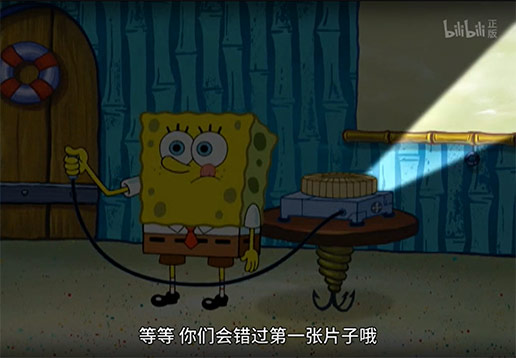
\includegraphics[width=0.88\linewidth]{project.jpg}
        \end{stampbox}
        \caption{投影放映}
      \end{figure}
    \end{column}
  \end{columns}
  \footnotetext{图像由 nickelodeon 持有版权。} % Overleaf 版本将会将图像设为 draft
\end{frame}

\begin{frame}
  \frametitle{什么是 beamer}

  \pkg{beamer} 是含有一些 PDF 交互式演示功能的文档类。

  \begin{figure}
    \centering
    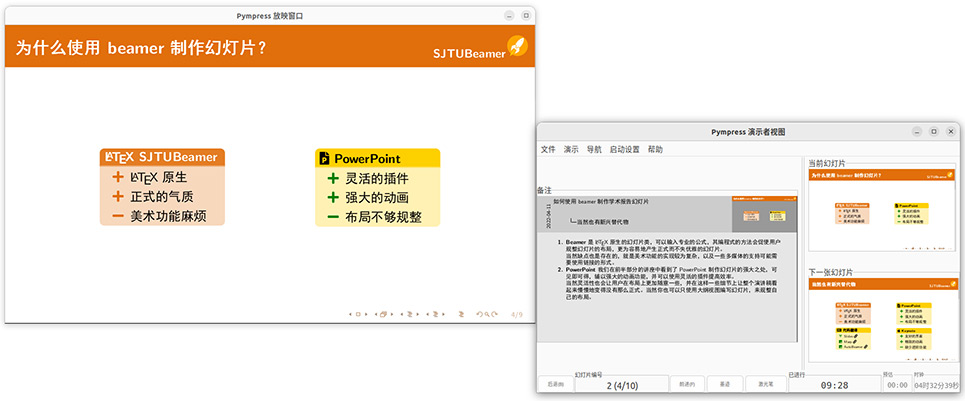
\includegraphics[width=0.7\linewidth]{pympress.jpg}
    \caption{Pympress 阅读器\footnote{需要使用 \cmd{note} 添加笔记,并在导言区添加 \cmd{setbeameroption\{notes on second screen\}} 以启用第二屏功能。} \link{https://github.com/Cimbali/pympress}}
    \note[item]{使用 Pympress 阅读器以最大化 beamer 的交互功能(左侧为放映窗口,右侧为演示者视图),并使用类似于 PowerPoint 演示者视图的界面方便演讲,可便携安装。我也参与了界面的汉化工作。}
  \end{figure}

\end{frame}

% beamer 基础

\begin{frame}
  \frametitle{简介}
  \begin{columns}
    \begin{column}{0.6\textwidth}
      \begin{itemize}
        \item 最早由谌翔于 2021 年 4 月发布
        \item 2021 年 5 月起由 SJTUG 接手,发布 1.0 版
        \item 2021 年 9 月李子龙重构了整个宏包的代码,升级版本号为 2.0
        \item 最新版:\SJTUBeamerVersion{} (\SJTUBeamerDate)
        \item 支持三种基本样式与扩展样式的幻灯片模板
        \item 支持镜像站克隆 \link{https://mirror.sjtu.edu.cn/git/SJTUBeamer.git/},支持使用任一引擎编译
      \end{itemize}
    \end{column}
    \begin{column}{0.4\textwidth}
      \begin{exampleblock}{}
        \begin{minipage}[c]{1cm}
          \includegraphics[width=0.8cm]{\getcontribpath{sjtug}{vi/sjtug}}
        \end{minipage}
        \begin{minipage}[c]{2cm}
          \href{https://github.com/sjtug}{sjtug}/\href{https://github.com/sjtug/SJTUBeamer}{SJTUBeamer}
        \end{minipage}
      \end{exampleblock}
      \vspace{-8pt}
      \begin{block}{}
        \scriptsize
        上海交通大学 Beamer 模版 | Beamer template for Shanghai Jiao Tong University
      \end{block}
      \vspace{-8pt}
      \begin{alertblock}{}
        \scriptsize
        \begin{tabular}{cl}
          \faStar       & 223 \\
          \faEye        & 6   \\
          \faCodeBranch & 13  \\
        \end{tabular}
      \end{alertblock}
    \end{column}
  \end{columns}
\end{frame}

\begin{frame}
  \frametitle{符合交大视觉形象识别系统}

  \begin{table}
    \caption{上海交通大学视觉形象识别系统规范(节选)}
    \vspace*{-5pt}
    \begin{stampbox}
      \footnotesize
      \begin{tabular}{llll}
        \alert{编号}                                                   & \alert{说明}                   & \alert{编号}                                                   & \alert{说明}     \\
        \href{https://vi.sjtu.edu.cn/index.php/articles/base/1}{A1-06} & 校徽需 $\frac{1}{5}h$ 安全空间 & \href{https://vi.sjtu.edu.cn/index.php/articles/base/5}{A5-03} & 辅助图形使用规范 \\
        \href{https://vi.sjtu.edu.cn/index.php/articles/base/3}{A3-01} & 标准色规范(含色阶)           & \href{https://vi.sjtu.edu.cn/index.php/articles/base/5}{A5-05} & 辅助图形底纹制作 \\
        \href{https://vi.sjtu.edu.cn/index.php/articles/base/3}{A3-02} & 辅助色彩规范(含色阶)         & \href{https://vi.sjtu.edu.cn/index.php/articles/app/7}{B1-01}  & 名片             \\
        \href{https://vi.sjtu.edu.cn/index.php/articles/base/3}{A3-05} & 品牌专用色彩搭配表             & \href{https://vi.sjtu.edu.cn/index.php/articles/app/7}{B1-20}  & 文件封套         \\
        \href{https://vi.sjtu.edu.cn/index.php/articles/base/4}{A4-08} & 二级机构中英文名称横式组合     & \href{https://vi.sjtu.edu.cn/index.php/articles/app/8}{B2-02}  & PPT 模板         \\
      \end{tabular}
    \end{stampbox}
  \end{table}

  正如 \textsc{SJTUThesis} 需要依照学位论文规范一样,\textsc{SJTUBeamer} 借助于 \TikZ{} 实现了《上海交通大学视觉形象识别系统》\link{https://vi.sjtu.edu.cn/} 的绝大部分规范\footnote{使用规范所规定的用品需要遵守相关许可条例 \link{https://vi.sjtu.edu.cn/index.php/articles/bulletin/16}。}。

  \note[item]{我相信小米的二百万 logo 更改让大家意识到了视觉形象识别系统的存在。交大在 2016 年的时候颁布了自己的视觉形象识别系统,并配套了对应的 PPT 模板。}

  \note[item]{许可条例第十三条规定:“校属各单位及个人可以自行或委托其他单位制作《手册》中有明确范例的物品,须严格遵照《手册》的要求,不得自行改动”,\textsc{SJTUBeamer} 也就需要依照该规范制作产物。}
\end{frame}

% SJTUBeamer 特殊宏